\sectioncounter{33}

\section{线面平行与面面平行}

\subsection{知识梳理}
线面平行判定定理: 平面外一条直线与此平面内的一条直线平行, 则前者与此平面平行.

对应的符号语言 (图 \ref{fig-190630-1800}): $a\not\subset\alpha$, 
$b\subset\alpha$ 且 $a\parallel b$ $\Rightarrow$ $a\parallel\alpha$.

面面平行判定定理: 一个平面内的两条相交直线与另一个平面平行, 则这两个平面平行.

对应的符号语言 (图 \ref{fig-190630-1810}): $a\subset\beta$, 
$b\subset\beta$, $a\cap b= P$, $a\parallel\alpha$, $b\parallel\alpha$ 
$\Rightarrow$ $\beta\parallel\alpha$.

推论 (补图): 若两个平面内有两组相交直线分别平行, 则这两个平面平行.

    \begin{figure}[htb]
    \small
    \centering
    \begin{minipage}[b]{0.45\linewidth}
      \centering
      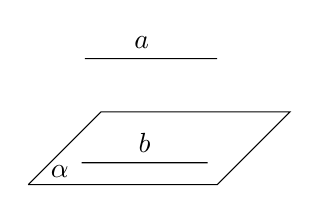
\begin{tikzpicture}[scale=0.8]
        \draw (0,0,0) coordinate (A);
        \draw (3,0,0) coordinate (B);
        \draw (0,0,-3) coordinate (D);
        \draw (B)++(D) coordinate (C);
        \draw (0.5,0) +(0,-0.05)node[above] {$\alpha$};
        
        \def\ay{2} \def\bz{-0.9}
        \draw (A)--(B)--(C)--(D)--(A) (0.5,0,\bz)--(2.5,0,\bz) (0.9,\ay)--(3,\ay);
        \draw (1.8,\ay) node[above] {$a$};
        \draw (1.5,0,\bz) node[above] {$b$};
      \end{tikzpicture}
      \caption{}\label{fig-190630-1800}
    \end{minipage}
    \hskip 0.5cm  
    \begin{minipage}[b]{0.45\linewidth}
      \centering
      \begin{tikzpicture}[scale=0.8]
        \draw (0,0,0) coordinate (A);
        \draw (3,0,0) coordinate (B);
        \draw (0,0,-3) coordinate (D);
        \draw (B)++(D) coordinate (C);
        \draw (0.5,0) +(0,-0.05)node[above] {$\alpha$};
        \draw (0,2,0) coordinate (A1);
        \draw (A1)++(B) coordinate (B1);
        \draw (A1)++(D) coordinate (D1);
        \draw (A1)++(C) coordinate (C1);
        \draw (A1)++(0.5,0) +(0,-0.05)node[above] {$\beta$};
        
        \draw (A)--(B)--(C)--(D)--(A) (A1)--(B1)--(C1)--(D1)--(A1);
        \draw[name path= linea] (0.7,2,-0.8)--(2.4,2,-2.1); % line a
        \draw[name path= lineb] (0.7,2,-2.1)--(2.4,2,-0.8); %\line b
        \draw (1.3,2,-0.7) node {$a$};
        \draw (0.5,2,-2.2) node {$b$}; 
        \draw[fill=black,name intersections={of=linea and lineb}] (intersection-1) circle (1pt) node[above] {$P$};
      \end{tikzpicture}
      \caption{}\label{fig-190630-1810}
    \end{minipage}
    \end{figure}

线面平行性质定理: 一条直线与一个平面平行, 
则过这条直线的任一平面与此平面的交线平行于该直线.

对应的符号语言 (图 \ref{fig-190630-1900}): $a\parallel\alpha$, 
$a\subset\beta$, $\alpha\cap\beta= b$ $\Rightarrow$ $a\parallel b$.

面面平行性质定理: 如果两个平行平面同时与第三个平面相交, 那么它们的交线平行.

对应的符号语言 (图 \ref{fig-190630-1910}): $\alpha\parallel\beta$, $\alpha\cap\gamma= a$, $\beta\cap\gamma= b$ $\Rightarrow$ $a\parallel b$.

    \begin{figure}[htb]
    \small
    \centering
    \begin{minipage}[b]{0.45\linewidth}
      \centering
      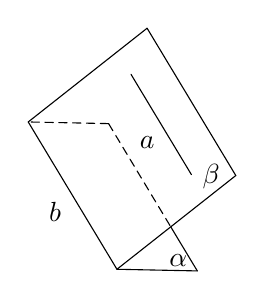
\begin{tikzpicture}[line cap=round,line join=round,scale=0.6]
        \draw (-2.796,-1.386)-- (-1.095,-1.421);
        \draw (-2.796,-1.386)-- (-4.674,1.732);
        \draw (-2.796,-1.386)-- (-0.280,0.598);
        \draw (-4.674,1.732)-- (-2.158,3.716);
        \draw (-2.158,3.716)-- (-0.280,0.598);
        \draw [densely dashed] (-2.973,1.697)-- (-4.674,1.732);
        \draw [densely dashed] (-2.973,1.697)-- (-1.657,-0.488);
        \draw (-1.657,-0.488)-- (-1.095,-1.421);
        \draw (-1.220,0.617)-- (-2.499,2.741);
        
        \draw (-1.5,-1.2) node {$\alpha$};
        \draw (-4.107,-0.163) node {$b$};
        \draw (-0.8,0.581) node {$\beta$};
        \draw (-2.158,1.289) node {$a$};
      \end{tikzpicture}
      \caption{}\label{fig-190630-1900}
    \end{minipage}
    \hskip 0.5cm  
    \begin{minipage}[b]{0.45\linewidth}
      \centering
      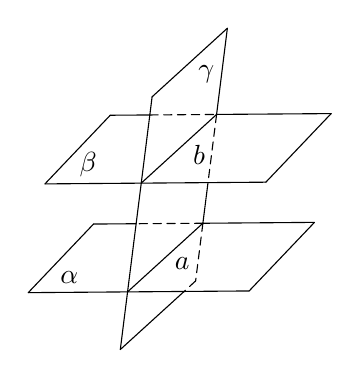
\begin{tikzpicture}[line cap=round,line join=round,scale=0.6]
        \draw (-4.071,-1.421)-- (0.605,-1.385);
        \draw (-4.071,-1.421)-- (-2.689,0.031);
        \draw (-2.122,-2.625)-- (-1.449,2.724);
        \draw (-1.449,2.724)-- (0.144,4.176);
        \draw (-3.717,0.881)-- (0.959,0.9175);
        \draw (0.959,0.9175)-- (2.341,2.369);
        \draw (-2.335,2.334)-- (-3.717,0.881);
        \draw (1.987,0.066)-- (0.605,-1.385);
        \draw (-1.679,0.897)-- (-0.084,2.351);
        \draw (-1.969,-1.405)-- (-0.374,0.048);
        \draw[densely dashed] (-1.497,2.340)-- (-0.084,2.351);
        \draw[densely dashed] (-0.084,2.351)-- (-0.266,0.907);
        \draw[densely dashed] (-0.374,0.048)-- (-0.528,-1.173);
        \draw[densely dashed] (-0.528,-1.173)-- (-0.772,-1.396);
        \draw (0.144,4.176)-- (-0.084,2.351);
        \draw (-0.266,0.907)-- (-0.374,0.048);
        \draw[densely dashed] (-0.374,0.048)-- (-1.787,0.038);
        \draw (-1.497,2.340)-- (-2.335,2.3344);
        \draw (-0.084,2.3515)-- (2.341,2.369);
        \draw (1.987,0.0666)-- (-0.374,0.048);
        \draw (-1.787,0.038)-- (-2.6896,0.031);
        \draw (-0.772,-1.396)-- (-2.122,-2.625);
        
        
        \draw (-3.2,-1.1) node {$\alpha$};
        \draw (-2.8,1.3) node {$\beta$};
        \draw (-0.3,3.2) node {$\gamma$};
        \draw (-0.457,1.5) node {$b$};
        \draw (-0.81,-0.8) node {$a$};
      \end{tikzpicture}
      \caption{}\label{fig-190630-1910}
    \end{minipage}
    \end{figure}

\lianxi
\begin{exercise}
    长方体 $ABCD\text{--}A_1 B_1 C_1 D_1$ 的各侧面中, 与直线 $AB$ 平行的有几个\,?
\end{exercise}
\beginsolution
    $2$ 个.
\endsolution

\begin{exercise}
    在正六棱柱的表面中, 互相平行的平面有多少对\,?
\end{exercise}
\beginsolution
    $4$ 对, 含 $1$ 对上、下底面, $3$ 对侧面.
\endsolution

\begin{exercise}
    已知命题 $p$: 平行于同一条直线的两个平面平行, 命题 $q$: 垂直于同一条直线的两个平面平行, 判断命题 $p$, $q$ 的真假.
\end{exercise}
\beginsolution
    命题 $p$ 为假命题, 命题 $q$ 为真命题.
\endsolution

\subsection{要点导学\quad 各个击破}
\subsubsection{线面、面面平行的判定}
\begin{example}
    如图 \ref{fig-190701-1820} 中左图所示, 在等边 $\triangle ABC$ 中, $D$,$E$ 分别是 $AB$,$AC$ 边上的点, $AD=AE$, $F$ 是 $BC$ 上一点, $AF$ 与 $DE$ 交于点 $G$, 将 $\triangle ABF$ 沿 $AF$ 折起, 得到右图所示的三棱锥 $A\text{--}BCF$, 求证: $DE\parallel$ 平面 $BCF$.
\end{example}
\beginsolution
    由等边 $\triangle ABC$ 中 $AD=AE$ 得 $DE\parallel BC$, 翻折后 $DG\parallel BF$ 且 $GE\parallel FC$, 所以平面 $DEG\parallel$ 平面 $BCF$. 因为平面 $ABC$ 与平面 $DEG$ 和平面 $BCF$ 分别交于 $DE$ 和 $BC$, 所以 $DE\parallel BC$, 从而 $DE\parallel$ 平面 $BCF$.
\endsolution

    \begin{figure}[htb]
    \small
    \centering
    \begin{minipage}[b]{0.45\linewidth}
      \centering
      \begin{tikzpicture}[line cap=round,line join=round,scale=1.2]
        \draw (-2,1.732) coordinate (A1) node[above] {$A$}
          (-3,0) coordinate (B1) node[below] {$B$}
          (-1,0) coordinate (C1) node[below] {$C$}
          ($(B1)!0.5!(C1)$) coordinate (F1) node[below] {$F$}
          ($(A1)!0.7!(B1)$) coordinate (D1) node[left] {$D$}
          ($(A1)!0.7!(C1)$) coordinate (E1) node[right] {$E$}
          ($(A1)!0.7!(F1)$) coordinate (G1) node[anchor=south east] {$G$};
        
        \draw (A1)--(B1)--(C1)--(A1)--(F1) (D1)--(E1);
        \draw[->] (-0.8,0.9)--(-0.2,0.9);
        
        \draw (0,1.5,-1.3) coordinate (A) node[above] {$A$}
          (0,0,0) coordinate (B) node[below] {$B$}
          (1.1,0,-1.3) coordinate (C) node[below] {$C$}
          (0,0,-1.3) coordinate (F) node[below] {$F$}
          ($(A)!0.7!(B)$) coordinate (D) node[left] {$D$}
          ($(A)!0.7!(C)$) coordinate (E) node[anchor=south west] {$E$}
          ($(A)!0.7!(F)$) coordinate (G) node[anchor=south west] {$G$};
        \draw (A)--(B)--(C)--(A) (D)--(E);
        \draw [densely dashed] (A)--(F)--(B) (C)--(F) (D)--(G)--(E);
      \end{tikzpicture}
      \caption{}\label{fig-190701-1820}
    \end{minipage}
    \hskip 0.5cm  
    \begin{minipage}[b]{0.45\linewidth}
      \centering
    %   \begin{tikzpicture}[line cap=round,line join=round,scale=1.2]        
    %     \draw (-0.4,0,-1) coordinate (A) node[left] {$A$}
    %       (0.5,0,0) coordinate (B) node[below] {$B$}
    %       (1.8,0,0) coordinate (C) node[below] {$C$}
    %       (2.2,0,-1) coordinate (D) node[right] {$D$}
    %       ($(A)!0.5!(D)$) coordinate (E) +(0,0,0.1) node[below] {$E$}
    %       (1.2,1.7,-0.8) coordinate (P) node[above] {$P$}
    %       ($(P)!0.5!(C)$) coordinate (F) node[right] {$F$};
          
    %     \draw (F)--(B)--(P)--(C)--(B)--(A)--(P)--(C)--(D)--(P);
    %     \draw [densely dashed] (A)--(D) (B)--(E)--(F);
    %   \end{tikzpicture}
        \includegraphics[scale=1.3]{2021-0829-1620-crop}
      \caption{}\label{fig-190701-1830}
    \end{minipage}
    \end{figure}

\begin{example}
    如图 \ref{fig-190701-1840} 所示, 在四棱锥 $P\text{--}ABCD$ 中, $AD\parallel BC$, $BC=\dfrac12 AD$, $E$,$F$ 分别为线段 $AD$,$PC$ 的中点, 求证: $AP\parallel$ 平面 $BEF$.
\end{example}
\beginsolution
    连接 $AC$ 交 $BE$ 于点 $G$, 再连接 $EC$, $GF$. 
    \mymarginpar{\begin{center}
        \includegraphics[scale=1.3,align=t]{2021-0829-1625-crop}
    \end{center}}
    由题意, $BC=AE$ 且 $BC\parallel AE$, 则四边形 $ABCE$ 为平行四边形, 所以 $AC$, $BE$ 互相平分, 即点 $E$ 为 $AC$ 的中点. 又因为 $F$ 为 $PC$ 的中点, 所以 $GF\parallel AP$, 故 $AP\parallel$ 平面 $BEF$.
\endsolution
       
\lianxi
\begin{exercise}[s]
    如图 \ref{fig-190701-1830} 所示, 在四棱锥 $E\text{--}ABCD$ 中, $\triangle ABD$ 为正三角形, $AB\perp BC$ 且 $M$,$N$ 分别为线段 $AE$,$AB$ 的中点, 求证: 平面 $DMN\parallel$平面 $BEC$.
\end{exercise}
\beginsolution
    因为 $DN$ 为正 $\triangle ABD$ 的中线, 所以 $DN\perp AB$. 由 $AB\perp BC$ 知, $DN\parallel BC$. 因为 $M$,$N$ 分别为线段 $AE$,$AB$ 的中点, 所以 $MN\parallel EB$, 故平面 $DMN\parallel$平面 $BEC$.
\endsolution

    \begin{figure}[htb]
    \small
    \centering
    \begin{minipage}[b]{0.45\linewidth}
      \centering
      \begin{tikzpicture}[line cap=round,line join=round,scale=1.2]
        \draw (0,0,0) coordinate (A) node[below] {$A$}
          (2,0,0) coordinate (B) node[below] {$B$}
          (1,0,-1.732) coordinate (D) +(0.1,0.1) node[anchor=south east] {$D$}
          (2,0,-1.5) coordinate (C) node[right] {$C$}
          (1.3,1.5,-1.3) coordinate (E) node[above] {$E$}
          ($(A)!0.5!(E)$) coordinate (M) node[anchor=south east] {$M$}
          ($(A)!0.5!(B)$) coordinate (N) node[below] {$N$};
        \draw (B)--(A)--(E)--(B)--(C)--(E) (M)--(N);
        \draw [densely dashed] (A)--(D)--(N) (C)--(D)--(B) (E)--(D)--(M);
      \end{tikzpicture}
      \caption{}\label{fig-190701-1840}
    \end{minipage}
    \hskip 0.5cm  
    \begin{minipage}[b]{0.45\linewidth}
      \centering
    %   \begin{tikzpicture}[line cap=round,line join=round,scale=1.2]
    %     \draw (0,0,0) coordinate (A) node[left] {$A$}
    %       (0,0,2) coordinate (B) node[below] {$B$}
    %       (2,0,0) coordinate (D) node[right] {$D$}
    %       (B)++(D) coordinate (C) node[below] {$C$}
    %       (0.3,1.6,0.5) coordinate (P) node[above] {$P$}
    %       ($(P)!0.5!(C)$) coordinate (E) node[right] {$E$}
    %       ($(C)!0.25!(A)$) coordinate (F) +(0,0,0.1) node[left] {$F$};
          
    %     \draw (P)--(B)--(C)--(D)--(P)--(C);
    %     \draw [densely dashed] (P)--(A)--(B)--(D)--(A)--(C) (E)--(F);
    %   \end{tikzpicture}
      \includegraphics[scale=1.3]{2021-0829-1640-crop}
      \caption{}\label{fig-190701-1850}
    \end{minipage}
    \end{figure}

\subsubsection{线面平行的性质}
\begin{example}
    如图 \ref{fig-190701-1850} 所示, 在四棱锥 $P\text{--}ABCD$ 中, 底面 $ABCD$ 是平行四边形, $E$ 为 $PC$ 的中点, $F$ 为线段 $AC$ 上一点. 若 $EF\parallel$ 平面 $PBD$, 求 $\dfrac{AF}{FC}$ 的值.
\end{example}
\beginsolution
    设 $AC$,$BD$ 交于点 $G$, 连接 $PG$, 
    \mymarginpar{\begin{center}
        \includegraphics[scale=1.3,align=t]{2021-0829-1645-crop}
    \end{center}}
    则 $G$ 为 $AC$ 的中点. 因为 $EF\parallel$ 平面 $PBD$, 所以 $EF\parallel PG$. 而 $E$ 为 $PC$ 的中点, 所以 $F$ 为 $GC$ 中点, 则
    \[FC= \frac12GC= \frac14AC,\quad
        AF= AC- FC= \frac34AC,\]
    从而 $\dfrac{AF}{FC}= 3$.
\endsolution

\lianxi
\begin{exercise}[s]
    如图 \ref{fig-190701-1900} 所示, 在空间四边形 $ABCD$ 中, 点 $E$,$F$,$G$,$H$ 分别在 $AB$,$BC$,$CD$,$DA$ 上, 且四边形 $EFGH$ 为平行四边形, 求证: $AC\parallel$ 平面 $EFGH$.
\end{exercise}
\beginsolution
    因为四边形 $EFGH$ 为平行四边形, 所以 $EF\parallel HG$, 则 $EF\parallel$ 平面 $ACD$, 继而 $EF\parallel AC$, 故 $AC\parallel$ 平面 $EFGH$.
\endsolution

    \begin{figure}[htb]
    \small
    \centering
    \begin{minipage}[b]{0.45\linewidth}
      \centering
      \begin{tikzpicture}[line cap=round,line join=round,scale=1.2]
        \draw (0,0) coordinate (A) node[left] {$A$}
          (2.2,1.2) coordinate (B) node[right] {$B$}
          (1,-0.8) coordinate (C) node[below] {$C$}
          (2.5,0) coordinate (D) node[right] {$D$}
          ($(A)!0.5!(B)$) coordinate (E) node[above] {$E$}
          ($(B)!0.5!(C)$) coordinate (F) node[right] {$F$}
          ($(C)!0.5!(D)$) coordinate (G) node[below] {$G$}
          ($(D)!0.5!(A)$) coordinate (H) node[anchor=north east] {$H$};
          
        \draw[name path= BC] (B)--(C);
        \draw[densely dashed,name path=AD] (A)--(D);
        \draw[name intersections={of=BC and AD}] (intersection-1) coordinate (I);
        
        \draw (B)--(A)--(C)--(D)--(I) (E)--(F)--(G);
        \draw[densely dashed] (E)--(H)--(G);
      \end{tikzpicture}
      \caption{}\label{fig-190701-1900}
    \end{minipage}
    \hskip 0.5cm  
    \begin{minipage}[b]{0.45\linewidth}
      \centering
    %   \begin{tikzpicture}[line cap=round,line join=round,scale=1]
    %     \draw (0,0,0) coordinate (A) node[left] {$A$}
    %       (2,0,2) coordinate (B) node[below] {$B$}
    %       (2.2,0,0) coordinate (C) node[right] {$C$}
    %       (0,2.1,0) coordinate (A1) node[left] {$A_1$}
    %       (B)++(A1) coordinate (B1) node[anchor=north west] {$B_1$}
    %       (C)++(A1) coordinate (C1) node[right] {$C_1$}
    %       ($(B)!0.5!(C)$) coordinate (D) node[anchor=north west] {$D$}
    %       ($(C1)!0.5!(C)$) coordinate (E) node[right] {$E$}
    %       ($(B)!0.5!(A)$) coordinate (M) node[anchor=north east] {$M$};
          
    %     \draw (M)--(A1)--(A)--(B)--(C)--(C1)--(A1)--(B1)--(C1) (B1)--(B) (D)--(E);
    %     \draw [densely dashed] (A)--(C)--(M) (C)--(A1);
    %   \end{tikzpicture}
      \includegraphics[scale=1.3]{2021-0829-1720-crop}
      \caption{}\label{fig-190701-1910}
    \end{minipage}
    \end{figure}

\subsubsection{直线与平面平行的探索问题}
\begin{example}
    在如图 \ref{fig-190701-1910} 所示的三棱柱 $ABC\text{--}A_1B_1C_1$中, $D$,$E$ 分别为线段 $BC$,$CC_1$ 的中点, 在线段 $AB$ 上是否存在一点 $M$, 使 $DE\parallel$ 平面 $A_1 MC$?
\end{example}
\beginsolution
    当 $M$ 为 $AB$ 中点时, $DE\parallel$ 平面 $A_1 MC$, 
    \mymarginpar{\begin{center}
        \includegraphics[scale=1.3]{2021-0829-1725-crop}
    \end{center}}
    证明如下:

    连接 $BC_1$, 由 $D$,$E$ 分别为线段 $BC$,$CC_1$ 的中点知, $DE\parallel BC_1$. 再连接 $AC_1$, 设其与 $A_1C$ 交于点 $F$. 由四边形 $ACC_1 A_1$ 为平行四边形知, $F$ 为 $AC_1$ 中点. 连接 $MF$, 因为 $M$ 为 $AB$ 中点,
    \mymarginpar{也可由 $BC_1\parallel$ 平面 $A_1MC$ 知 $BC_1\parallel MF$, 则 $M$ 只能为 $AB$ 中点.}
    所以 $MF\parallel BC_1$, 则 $MF\parallel DE$, 故 $DE\parallel$ 平面 $A_1 MC$.

    \varexercise 条件“三棱柱 $ABC\text{--}A_1B_1C_1$”可减弱为“四边形 $ACC_1 A_1$ 为平行四边形”.

    \varexercise 若 $D$,$E$ 不再是中点, 只要 $DE\parallel BC_1$, 仍可得 $M$ 为 $AB$ 中点.

    \varexercise 若 $DE$ 不平行于 $BC_1$, 则用纯几何法确定点 $M$ 的位置仍可行, 但推理略复杂, 可改用空间向量法求解. 
    \mymarginpar{空间向量法原理是选定基向量后, 将某一向量用两种方式表示, 然后根据空间向量基本定理, 这两种表示法是同一种, 即基向量对应系数相等, 从而得到对应的方程组.}
    例如, 若将“点 $E$ 为线段 $CC_1$ 的中点”改为“点 $E$ 在线段 $CC_1$ 上且 $CE= 2EC_1$”, 则有如下解法 (以 $\overrightarrow{CA}$,$\overrightarrow{CB}$,$\overrightarrow{CC_1}$ 为空间基向量):

    为简化记号, 设 $\overrightarrow{CA}= \bm{a}$, $\overrightarrow{CB}= \bm{b}$, $\overrightarrow{CC_1}= \bm{c}$, 则 
    \[\overrightarrow{CD}= \frac12\bm{b},\quad
    \overrightarrow{CE}= \frac23\bm{c},\quad
    \overrightarrow{CA_1}= \bm{a}+ \bm{c},\]
    所以 $\overrightarrow{DE}= \overrightarrow{CE}- \overrightarrow{CD}= \dfrac23\bm{c}- \dfrac12\bm{b}$. 因为 $DE\parallel$ 平面 $A_1MC$, 所以 $\overrightarrow{CM}$,$\overrightarrow{CA_1}$,$\overrightarrow{DE}$ 共面, 即可用后两者表示 $\overrightarrow{CM}$. 设 $\overrightarrow{CM}= m\overrightarrow{CA_1}+ n\overrightarrow{DE}$, 则
    \[\begin{aligned}
        \overrightarrow{CM}
        &= m(\bm{a}+\bm{c})+ n\biggl(\frac23\bm{c}- \frac12\bm{b}\biggr)\\
        &= m\bm{a} - \frac{n}2\bm{b}+ \biggl(m+\frac23n\biggr)\bm{c}.
    \end{aligned}\]
    由点 $M$ 在 $AB$ 上可设 $\overrightarrow{AM}= \lambda\overrightarrow{MB}$, 则
    \[\begin{gathered}
        \overrightarrow{CM}- \overrightarrow{CA}
        = \lambda(\overrightarrow{CB}- \overrightarrow{CM}),\\
        \overrightarrow{CM}
        = \frac{\overrightarrow{CA}}{1+\lambda}
            + \frac{\lambda\overrightarrow{CB}}{1+\lambda}
        = \frac{\bm{a}}{1+\lambda}
            + \frac{\lambda\bm{b}}{1+\lambda}.
    \end{gathered}\]
    对比 $\overrightarrow{CM}$ 的两种表示可知,
    \[m= \frac1{1+\lambda},\quad
    -\frac{n}2= \frac{\lambda}{1+\lambda},\quad
    m+\frac23n= 0,\]
    消去 $m$,$n$ 可得
    \[\frac1{1+\lambda}- \frac43\cdot \frac{\lambda}{1+\lambda}=0,\]
    解得 $\lambda= \dfrac34$, 即当点 $M$ 满足 $AM= \dfrac34 MB$ 时符合题意.
\endsolution 
    
\lianxi
\begin{exercise}[s]
    在如图 \ref{fig-190701-1920} 所示的几何体中, $AC= \sqrt3$, $AB=2BC=2$, $AC\perp FB$.
    
    (1) 求证: $AC\perp FC$.
    
    (2) 线段 $AC$ 上是否存在点 $M$, 使 $EA\parallel$ 平面 $FDM$?
\end{exercise}
\beginsolution
    (1) 因为 $AC=\sqrt3$, $AB=2$, $BC=1$, 所以
    \[AB^2= AC^2+ BC^2,\quad\text{即}\quad AC\perp BC.\]
    而 $AC\perp FB$, 所以 $AC\perp$ 平面 $FBC$, 故 $AC\perp FC$.

    (2) 连接 $EC$ 交 $DF$ 于点 $G$, 则在平行四边形 $CDEF$ 中, $G$ 为 $EC$ 中点. 再连接 $GM$, 由 $EA\parallel$ 平面 $FDM$ 知 $EA\parallel Gm$, 故 $M$ 为 $AC$ 中点.
\endsolution

    \begin{figure}[htb]
    \small
    \centering
    \begin{minipage}[b]{0.45\linewidth}
      \centering
      \begin{tikzpicture}[line cap=round,line join=round,scale=1.6]        
        \draw (0,0,0) coordinate (D) node[anchor=south east] {$D$}
          (1,0,0) coordinate (C) node[anchor=south east] {$C$}
          (-0.5,0,0.866) coordinate (A) node[below] {$A$}
          ($(A)+2*(C)$) coordinate (B) node[below] {$B$}
          (0,1,0) coordinate (E) node[left] {$E$}
          (C)++(E) coordinate (F) node[right] {$F$};
        
        \draw (A)--(B)--(F)--(E)--(A);
        \draw[densely dashed] (E)--(D)--(A)--(C)--(B)--(D)--(C)--(F)--(D);
      \end{tikzpicture}
      \caption{}\label{fig-190701-1920}
    \end{minipage}
    \hskip 0.5cm  
    \begin{minipage}[b]{0.45\linewidth}
      \centering
      \begin{tikzpicture}[line cap=round,line join=round,scale=0.9]
        \draw (0,0,0) coordinate (D) node[left] {$D$}
          (0,0,2) coordinate (A) node[below] {$A$}
          (2,0,0) coordinate (C) node[right] {$C$}
          (0,2,0) coordinate (D1) node[left] {$D_1$}
          (A)++(C) coordinate (B) node[below] {$B$}
          (A)++(D1) coordinate (A1) node[left] {$A_1$}
          (C)++(D1) coordinate (C1) node[right] {$C_1$}
          (C)++(D1)++(A) coordinate (B1) +(0,0,0.1) node[right] {$B_1$}
          ($(B)!0.5!(A)$) coordinate (E) node[below] {$E$}
          ($(D1)!0.5!(C)$) coordinate (M) +(0,0,0.1) node[left] {$M$};
          
        \draw (A1)--(A)--(B)--(C)--(C1)--(D1)--(A1)--(B1)--(C1) (B)--(B1);
        \draw [densely dashed] (D)--(A)--(D1)--(D)--(C)--(D1) (E)--(M);
      \end{tikzpicture}
      \caption{}\label{fig-190701-1930}
    \end{minipage}
    \end{figure}

\subsubsection{课堂评价}
\begin{exercise}
    平面 $\alpha$ 内的两条直线 $a$,$b$ 都平行于平面 $\beta$, 判断 $\alpha$ 和 $\beta$ 的位置关系.
\end{exercise}
\beginsolution
    若 $a$ 与 $b$ 相交, 则 $\alpha\parallel \beta$; 若 $a\parallel b$, 则 $\alpha\parallel \beta$ 或 $\alpha$ 与 $\beta$ 相交.
\endsolution

\begin{exercise}
    如图 \ref{fig-190701-1930} 所示, 在长方体 $ABCD\text{--}A_1 B_1 C_1 D_1$ 中, 点 $E$ 是线段 $AB$ 上的动点, 点 $M$ 为 $D_1C$ 的中点. 求证: $ME\parallel$ 平面 $ADD_1 A_1$ 的充要条件是 $E$ 为 $AB$ 的中点.
\end{exercise}
\beginsolution
    连接 $AD$, $AC$, 取 $AC$ 中点 $F$, 连接 $MF$. 由 $M$ 为 $D_1C$ 的中点知, $MF\parallel AD_1$. 连接 $EF$, 则 $ME\parallel$ 平面 $ADD_1A_1$ 等价于平面 $MEF\parallel$ 平面 $ADD_1A_1$, 又等价于 $EF\parallel AD$, 即 $EF\parallel DC$, 所以 $E$ 为 $AB$ 的中点.
\endsolution

\subsection{课后练习}

\begin{exercise}
    判断下列命题是否正确:
    
    (1) 若直线 $l$ 上有无数个点不在平面 $\alpha$ 内, 则 $l\parallel \alpha$;
    
    (2) 若直线 $l$ 与平面 $\alpha$ 平行, 则 $l$ 与平面 $\alpha$ 内的任意一条直线都平行;
    
    (3) 若直线 $a\parallel b$, $a\parallel$ 平面 $\alpha$, 则$b\parallel$ 平面 $\alpha$;
    
    (4) 若直线 $l\parallel$ 平面 $\alpha$, 则 $l$ 与 $\alpha$ 
    内的任意直线都没有公共点.
\end{exercise}
\beginsolution
    (1) 错误, $l$ 与 $\alpha$ 可能相交.

    (2) 错误, 线面平行时, 线与面内的直线可能异面.

    (3) 错误, 可能 $b\subset\alpha$.

    (4) 正确, 可利用反证法说明.
\endsolution

\begin{exercise}
    在下列条件中, 哪些可以判定平面 $\alpha\parallel$ 平面 $\beta$?
    
    (1) $\alpha$, $\beta$ 都垂直于平面 $\gamma$;
    
    (2) $\alpha$ 内不共线的三个点到 $\beta$ 的距离相等;
    
    (3) $l, m$ 是 $\alpha$ 内两条直线, 且 $l\parallel \beta$, $m\parallel \beta$;
    
    (4) $l, m$ 是两条异面直线, 且 $l\parallel \alpha$, $m\parallel \alpha$, $l\parallel \beta$, $m\parallel \beta$.
\end{exercise}
\beginsolution
    (1) 不可以, 参考墙角处三个面的位置关系.

    (2) 不可以, 可能有两个点与第三个点在 $\beta$ 异侧.

    (3) 不可以, 还需要 $l,m$ 相交.

    (4) 可以, $l, m$ 可以平移至相交. 
\endsolution

\begin{exercise}
    如图 \ref{fig-190701-1940} 所示, 在四棱锥 $P\text{--}ABCD$ 中, $AB\parallel DC$, $AB\perp AD$, $BC=5$, $DC=3$, $AD=4$, $\angle PAD=60^\circ$. 若 $M$ 为 $PA$ 的中点, 求证: $DM\parallel$ 平面 $PBC$.
\end{exercise}
\beginsolution
    过点 $C$ 作 $CE\perp AB$ 于点 $E$, 则四边形 $AECD$ 为矩形, 
    \[AE=DC=3,\quad CE=AD=4.\]
    因为 $CB=5$, 所以 $EB=3$, 则 $AB=6= 2DC$. 取 $PB$ 中点 $F$, 连接 $MF$, 由 $M$ 为 $PA$ 的中点知,
    \[MF\parallel AB\parallel DC,\quad MF= \frac12 AB= DC.\]
    连接 $CF$, 则四边形 $MDCF$ 为平行四边形, 所以 $MD\parallel CF$, 即 $DM\parallel$ 平面 $PBC$.
\endsolution

    \begin{figure}[htb]
    \small
    \centering
    \begin{minipage}[b]{0.45\linewidth}
      \centering
      \begin{tikzpicture}[line cap=round,line join=round,scale=0.4]        
        \draw (0,0,0) coordinate (D) node[anchor=south west] {$D$}
          (3,0,0) coordinate (C) +(-0.2,0,0) node[anchor=south east] {$C$}
          (0,0,4) coordinate (A) node[below] {$A$}
          ($(A)+2*(C)$) coordinate (B) node[below] {$B$}
          (2,6,2) coordinate (P) node[left] {$P$}
          ($(A)!0.5!(P)$) coordinate (M) node[left] {$M$};
        
        \draw (A)--(B)--(P)--(A);
        \draw[densely dashed] (P)--(D)--(M) (A)--(D)--(C) (B)--(C)--(P);
      \end{tikzpicture}
      \caption{}\label{fig-190701-1940}
    \end{minipage}
    \hskip 0.5cm  
    \begin{minipage}[b]{0.45\linewidth}
      \centering
      \begin{tikzpicture}[line cap=round,line join=round,scale=0.9]
        \draw (0,0,0) coordinate (A) node[left] {$A$}
          (1,0,1.732) coordinate (B) node[below] {$B$}
          (4,0,0) coordinate (C) node[right] {$C$}
          (0,2,0) coordinate (P) node[left] {$P$}
          ($(B)!0.5!(P)$) coordinate (D) node[right] {$D$}
          ($(B)!0.5!(C)$) coordinate (E) node[below] {$E$}
          ($(A)!0.333!(C)$) coordinate (F) node[below] {$F$};
          
        \draw (D)--(A)--(P)--(B)--(A) (B)--(C)--(P)--(E);
        \draw [densely dashed] (A)--(C) (P)--(F)--(E);
      \end{tikzpicture}
      \caption{}\label{fig-190701-1950}
    \end{minipage}
    \end{figure}

\begin{exercise}
    如图 \ref{fig-190701-1950} 所示, 在三棱锥 $P\text{--}ABC$ 中, $BC\perp\text{平面\ }PAB$. 已知 $PA=AB$, $D, E$ 分别为 $PB, BC$ 的中点.
    
    (1) 求证: $AD\perp$ 平面 $PBC$;
    
    (2) 若点 $F$ 在线段 $AC$ 上, 满足 $AD\parallel$ 平面 $PEF$, 求 $\dfrac{AF}{FC}$ 的值.
\end{exercise}
\beginsolution
    (1) 因为 $BC\perp$ 平面  $PAB$, 所以 $BC\perp AD$. 又因为 $PA=AB$, $D$ 为 $PB$ 的中点, 所以 $AD\perp PB$, 则 $AD\perp$ 平面 $PBC$.

    (2) 连接 $CD$ 与 $PE$ 相交, 设交点为点 $G$, 连接 $DE$. 
    \mymarginpar{此小题也可用空间向量法求解 (以 $\overrightarrow{AB},\overrightarrow{AC},\overrightarrow{AP}$ 为基向量).}
    因为 $D, E$ 分别为 $PB, BC$ 的中点, 所以 $DE\parallel PC$, $DE= \dfrac12 PC$, 则 
    \[\triangle DGE\sim \triangle CBP,\quad DG=\frac12 GC.\]
    连接 $PG$, 由 $AD\parallel$ 平面 $PEF$ 知 $AD\parallel FG$, 则
    \[\frac{AF}{FC}= \frac{DG}{GC}= \frac12.\]
\endsolution

\begin{exercise}
    已知圆 $O$ 的直径 $AB=4$, 点 $C, D$ 是圆 $O$ 上位于 $AB$ 两侧的两点, 且 $\angle CAB=45^\circ$, $\angle DAB=60^\circ$, $F$ 为弧 $BC$ 的中点. 将圆 $O$ 沿直径 $AB$ 折起, 使两个半圆所在的平面互相垂直.
    
    (1) 求证: $OF\parallel AC$.
    
    (2) 在弧 $BD$ 上是否存在点 $G$, 使得 $FG\parallel$ 平面 $ACD$?
\end{exercise}
\beginsolution
    (1) 连接 $CO$, 则 $\angle COB= 2\angle CAB= 90^\circ$. 由 $F$ 为弧 $BC$ 的中点知, $\angle FOB= \dfrac12\angle COB= 45^\circ$, 故 $\angle FOB= \angle CAB$, $OF\parallel AC$.
    
    (2) 连接 $OG$, 类似于 (1) 可证, 
    \mymarginpar{此时 $FG$ 与 $CD$ 不平行 (为什么?).}
    当 $G$ 为弧 $BD$ 的中点时, $OG\parallel AD$, 则平面 $ACD\parallel$ 平面 $OFG$, 所以 $FG\parallel$ 平面 $ACD$.
\endsolution